% !TeX root = ../thesis.tex

\chapter{Evaluation}
\label{sec:evaluation}
In diesem Kapitel findet die Evaluation des in Kapitel~\ref{sec:concepts} vorgestellten Ansatzes statt.
Zun\"achst werden die Szenarien vorgestellt, anhand denen der Ansatz evaluiert wird.
Anschlie{\ss}end wird auf die Implementierung des Ansatzes eingegangen.
Schlussendlich werden die Simulationsergebnisse vorgestellt und diskutiert. 
Dabei werden zun\"achst die Ergebnisse eines einzelnen Planungsschrittes untersucht.
Anschlie{\ss}end wird das verhalten des Ego"=Fahrzeuges bei einer fortlaufenden Neuplanung der Trajektorie betrachtet.


\section{Auswahl der Simulationsszenarien}
Der in Kapitel~\ref{sec:concepts} vorgestellte Ansatz soll simulativ getestet werden.
Da es im Rahmen dieser Arbeit zeitlich nicht m\"oglich ist alle Fahrstreifenwechselszenarien abzudecken, wird sich auf einige beispielhafte Szenarien beschr\"ankt.
Diese Szenarien soll die wichtigsten Aspekte des Ansatzes abdecken.

Ein Fahrstreifenwechselszenario bei dem sich am Ende des aktuellen Fahrstreifen nach dem Rei{\ss}verschlussverfahren auf dem neuen Fahrstreifen eingeordnet werden muss ist das einfachste Szenario.
Der Zeitpunkt an dem der Fahrstreifenwechsel eingeleitet werden sollte ist weitestgehend vorgegeben.
Es ist au{\ss}erdem in der Regel klar welche L\"ucke f\"ur den Fahrstreifenwechsel gew\"ahlt wird und es ist klar geregelt wie sich die Fahrzeuge zu verhalten haben.
Eine solche Verkehrssituation kann h\"aufig auch ohne einen kooperativen Ansatz gel\"ost werden. 
Ein freiwilliger Fahrstreifenwechsel, bei dem ein langsameres Fahrzeug \"uberholt werden soll stellt bereits eine schwierigere Aufgabe dar. 
Es muss zuerst eine geeignete L\"ucke ausgew\"ahlt werden.
Anschlie{\ss}end muss f\"ur diese L\"ucke ein Fahrstreifenwechsel geplant und ausgef\"uhrt werden.
Allerdings ist ein automatisiertes Fahrzeug in der Regel nicht auf den Fahrstreifenwechsel angewiesen.
Der Fahrstreifenwechsel kann so lange herausgez\"ogert werden bis sich eine L\"ucke ergibt, die gro{\ss} genug ist um einen Fahrstreifenwechsel durchzuf\"uhren, bei dem kein kooperatives Verhalten verlangt ist.
Dadurch muss das Fahrzeug zwar f\"ur eine gewisse Zeit von seiner Wunschgeschwindigkeit abweichen, es kommt aber in der Regel nicht zum Stillstand und stellt damit auch kein Sicherheitsrisiko dar.

Aus diesem Grund werden bei der Evaluierung ausschlie{\ss}lich Szenarien betrachtet, in denen ein notwendiger Fahrstreifenwechsel ausgef\"uhrt wird.
Bei einem solchen Szenario ist in der Regel vorgegeben ab wann der Fahrstreifenwechsel ausgef\"uhrt werden kann und bis wann er sp\"atestens vollzogen sein muss.
Um ein Stehenbleiben auf dem aktuellen Fahrstreifen zu vermeiden muss bei dichtem Verkehr deshalb in der Regel ein Fahrstreifenwechsel ausgef\"uhrt werden, der ein kooperatives Fahrverhalten verlangt.
Eine solches Szenario ergibt sich in der Haid"=und"=Neu"=Stra{\ss}e in Karlsruhe, Deutschland, die in der simulativen Evaluierung genutzt wurde.
Fahrzeuge die Links abbiegen wollen und auf dem rechten Fahrstreifen fahren, m\"ussen den Fahrstriefenwechsel vollzogen haben, bevor sich die beiden Fahrstreifen trennen (siehe Abbildung~\ref{fig:Szene}).

\begin{figure}[!htbp]
    \centering
    \subfigure[Darstellung der Haid"=und"=Neu"=Stra{\ss}e in Google Maps \gls{hun}. In rot dargestellt der aktuelle Fahrstreifen des Ego"=Fahrzeuges und in blau der Zielfahrstreifen]{
        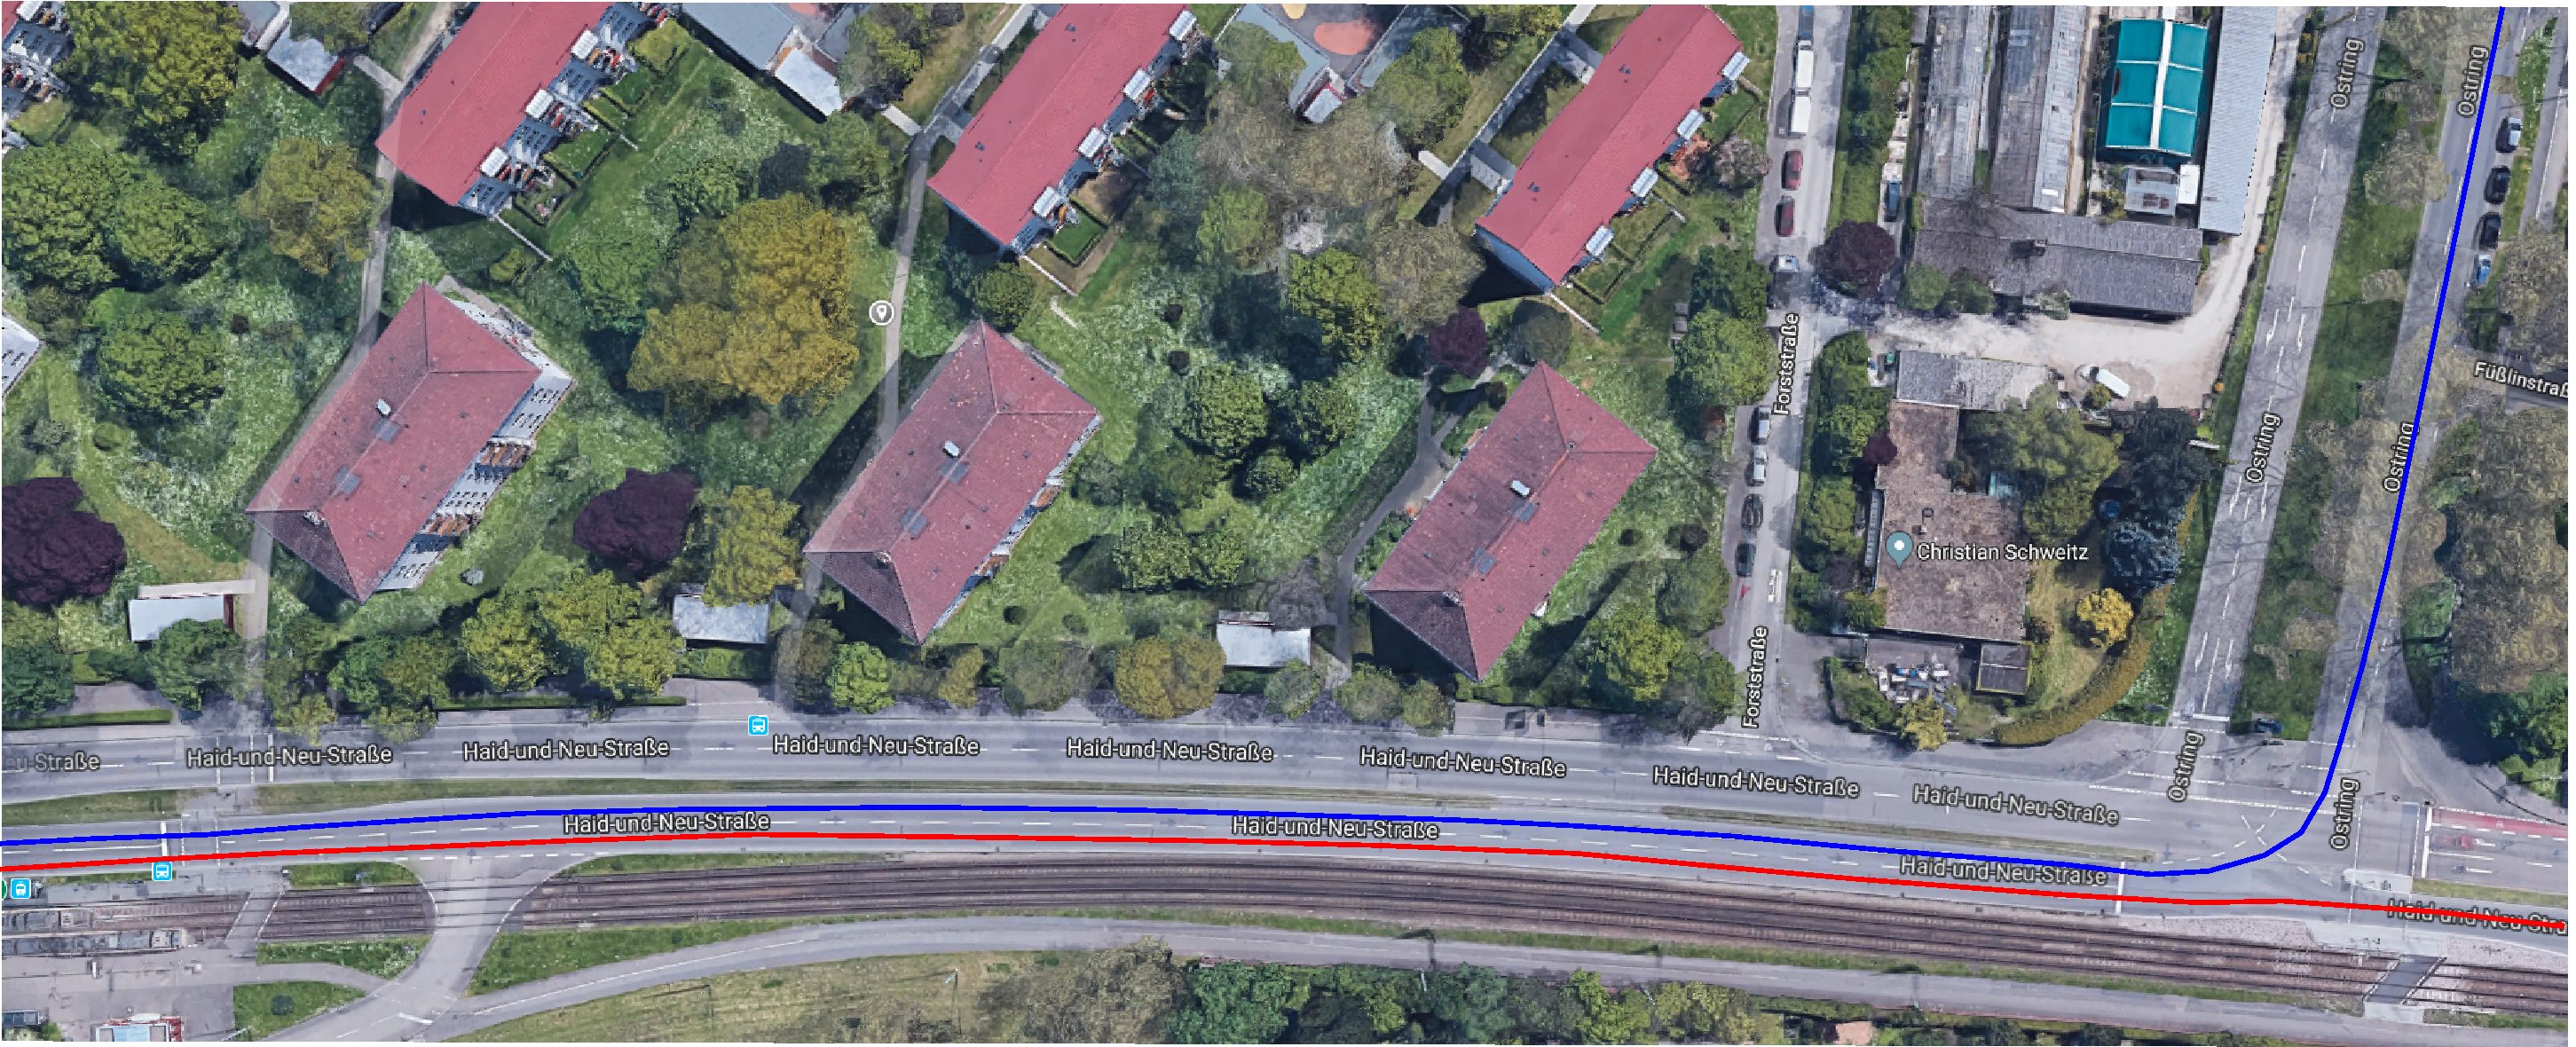
\includegraphics[width =  0.85 \textwidth]{maps.pdf}
        \label{google}
    }
    \subfigure[Darstellung der Haid"=und"=Neu"=Stra{\ss}e in der Simulationsumgebung \gls{ros} basierend auf den Datengrundlagen des Open"=Source"=Karten"=Framework lanelet2]{
        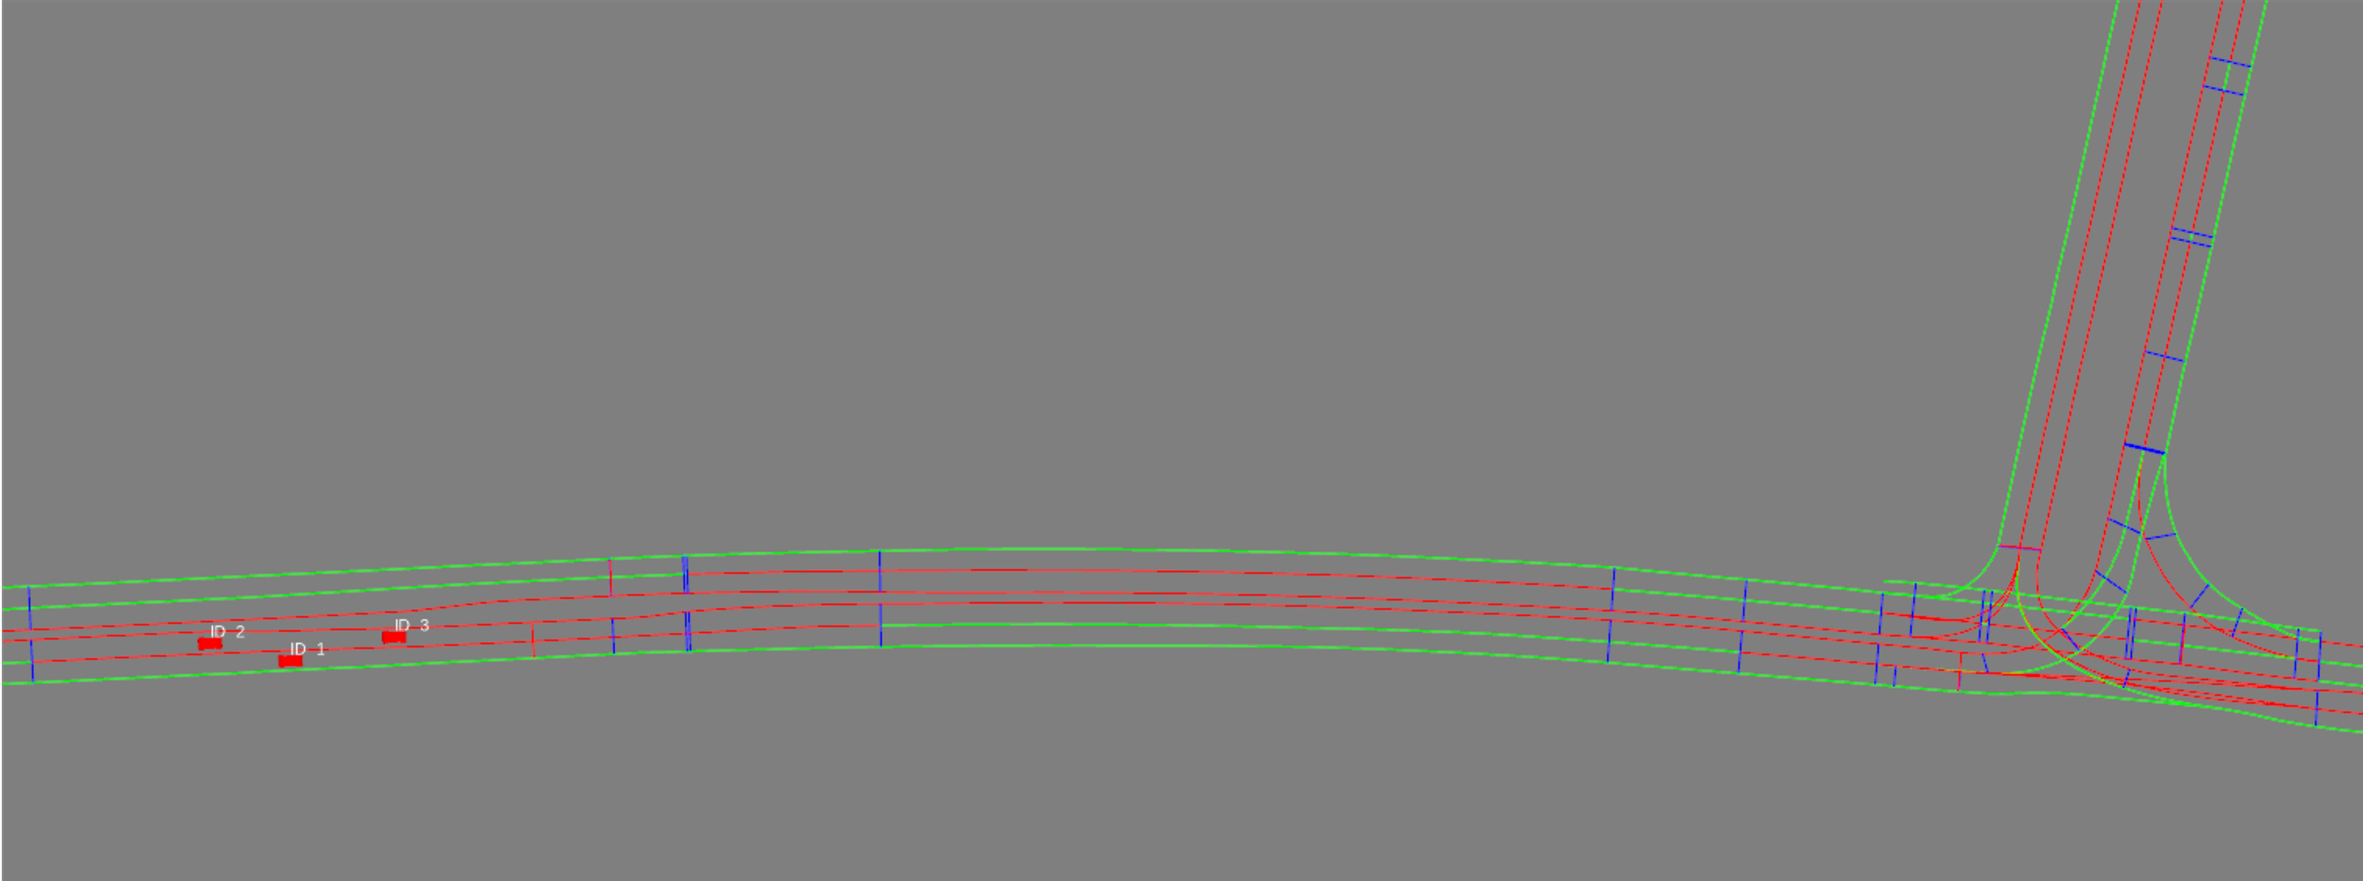
\includegraphics[width =  0.85 \textwidth]{rviz_sce.pdf}
        \label{rviz}
    }
    \caption[Haid-und-Neu"=stra{\ss}e]{Haid"=und"=Neu"=Stra{\ss}e in Karlsruhe}
    \label{fig:Szene}
\end{figure}


\section{Implementierung}
Die Implementierung des Ansatzes fand in der Programmiersprache Python statt.
Der implementierte Ansatz wurde dann in einer \gls{ros}"=Simulationsumgebung eingebunden.
Stra{\ss}eninformationen wie der Verlauf der Referenzkurve und der Fahrstreifen wurden dem von Poggenhans et al. \cite{Poggenhans2018} vorgestelltem Open"=Source"=Karten"=Framework lanelet2 entnommen.
Die Implementierung fand ausschlie{\ss}lich f\"ur die ausgew\"ahlten Szenarien statt.
Teilaspekte die f\"ur die Szenarien nicht relevant sind wurden ausgelassen.
So fand beispielsweise keine Implementierung eines zweifachen Fahrstreifenwechsels oder einer Pfadplanung f\"ur einen freiwilligen Fahrstreifenwechsel statt.
Es wurde bei der Implementierung darauf geachtet, dass der Quellecode modluar aufgebaut ist und somit die entsprechenden Module erg\"anzt werden k\"onnen.
Da der Fokus der Arbeit auf der Konzeptentwicklung liegt, wird im Folgenden nur eine kurze \"Ubersicht zur Implementierung gegeben.


\subsection{Objektorientierte Programmierung}
\label{sec:Objektorientiert}
Die Implementierung in Python fand objektorientiert statt.
Dies tr\"agt zur \"Ubersichtlichkeit des Quellcodes bei und sorgt daf\"ur, dass einzelne Modul leicht ausgetauscht werden k\"onnen.
Es wurden sowohl Klassen zur Beschreibung einzelner Simulationsemelemte als auch f\"ur einzelne Teilschritte des Planungsalgorihmus erstellt.

Klassen zur Beschreibung einzelner Simulationselemente:
\begin{itemize}
\item \textit{Vehicle}: Beschreibung der in der Simulation betrachteten Fahrzeuge. 
Es werden sowohl Informationen \"uber die geometrischen Abmessungen als auch \"uber den Anfangszustand des Fahrzeuges gegeben. 
Jedes Fahrzeug enth\"alt zus\"atzlich ein Objekt der Costfunctional"=Klasse. 
Durch dieses Objekt ist das fahrzeugspezifische Kostenfunktional gegeben.

\item \textit{StreetInfo}: Enth\"alt den Verlauf der Referenzkurve, sowie des aktuellen Fahrstreifens und des Zielfahrstreifens. 
Der aktuelle Fahrstreifen und der Zielfahrstreifen werden durch ein Objekt der Klasse Path beschrieben.
Es werden aus au{\ss}erdem die Informationen gegeben, ab welcher Wegstrecke \gls{symb:s_cs} entlang der Referenzkurve ein Fahrstreifenwechsel eingeleitet werden kann und bis zu welcher Wegstrecke \gls{symb:s_ce} er vollzogen sein muss.

\item \textit{Path}: Geometrische Beschreibung des Verlaufs des Pfades in Frenetkoordinaten.
Die Klasse enth\"alt au{\ss}erdem eine Methode zur Berechnung der Bewegung entlang der Referenzkurve bei gegebener Geschwindigkeit und Beschleunigung des Fahrzeuges.

\item \textit{Costfuntional}: Beschreibung des fahrzeugspezifischen Kostenfunktionals. 
Die Klasse enth\"alt f\"ur jeden Kostenterm (\gls{symb:G_v}, \gls{symb:G_a}, \gls{symb:G_sd}, \gls{symb:G_lc}, \gls{symb:G_lcend}) eine Methoden zur Berechnung der entsprechenden Kosten.
Hier konnte eine bereits vorhandene Klasse erweitert werden.
\end{itemize}

Klassen f\"ur einzelne Teilschritte:
\begin{itemize}
\item \textit{EgoIndependentPrediction}: Erzeugung einer vom Ego"=Fahrzeug unabh\"angigen Bewegungspr\"adiktion aller relevanten Fahrzeuge.
Die Pr\"adiktion findet basierende auf vorgegebenen Anfangszust\"anden der Fahrzeuge sowie deren gew\"unschten Optimalgeschwindigkeit statt.


\item \textit{CreateVelocityProfiles}: Erzeugung zuf\"alliger Geschwindigkeitsprofile. 
Basierend auf einem gegebenen Anfangszustand des Fahrzeuges werden zuf\"allige, diskrete Beschleunigungsverl\"aufe und die entsprechenden Geschwindigkeitsverl\"aufe erzeugt.
Dabei werden die Beschleunigungen und Geschwindigkeiten auf vorgegebene Extremwerte begrenzt.
Es konnte auf einer bestehenden Klasse aufgebaut werden.
 
\item \textit{GenerateCooperativeLaneChangeTrajectorySet}: Erzeugung eines Trajektoriensets f\"ur einen kooperativen Fahrstreifenwechsel.
F\"ur jedes Fahrzeug wird eine Trajektorie ermittelt.
Die Trajektorien werden aufgrund eines vorgegebenen Geschwindigkeitprofils des Ego"=Fahrzeuges und einer vom Ego"=Fahrzeug unabh\"angigen Bewegungspr\"adiktion der restlichen Fahrzeuge ermittelt.
Die Klasse enth\"alt jeweils ein Objekt der Klassen PlanLaneChangePath, Classification und InnerOptimization.

\item \textit{PlanLaneChangePath}: Ermittlung des Pfades f\"ur einen Fahrstreifenwechsel.
Der Pfad ergibt sich aus dem Pfad des aktuellen Fahrstreifens, dem Pfad des Zielfahrstreifens und dem Fahrstreifenwechselpfad.
Der sich ergebende Pfad wird \"uber ein Objekt der Klasse Path beschrieben.
Die Klasse enth\"alt au{\ss}erdem die Information zu welchem Zeitpunkt \(t_\mathrm{lc, start}\) der Fahrstreifenwechsel eingeleitet wird, zu welchem Zeitpunkt \gls{symb:t_lc} das Fahrzeuge auf den Zielfahrstreifen auff\"ahrt und zu welchem Zeitpunkt \(t_\mathrm{lc, end}\) der Fahrstreifenwechsel beendet wird.

\item \textit{Classification}: Klassifizierung der Fahrzeuge. 
Die Fahrzeuge werden aufgrund der vom Ego"=Fahrzeug unabh\"angigen Bewegungspr\"adiktion und einer gegeben Trajektorie des Ego"=Fahrzeuges in beteiligte, unbeteiligte und beeinflusste Fahrzeuge eingeteilt.

\item \textit{InnerOptimization}: Ermittlung einer kooperativen Fahrstreifenwechseltrajektorie eines beteiligten Fahrzeuges bei gegebener Trajektorie des Ego"=Fahrzeuges. 
Die L\"osung des inneren Optimierungsproblems findet durch einen samplingbasierten Ansatz statt, bei dem randomisierte Geschwindigkeitsprofile erzeugt werden.
Dazu wird ein Objekt der Klasse CreateVelocityProfiles erzeugt.


\end{itemize}

\subsection{Erzeugung randomisierter Geschwindigikeitsprofil}
Die Erzeugung der randomisierten Geschwindigkeitsprofile findet in der in Kapitel~\ref{sec:Objektorientiert} vorgestellten Klasse CreateVelocityProfiles statt.
Dabei wird f\"ur jeden einzelnen Zeitschritt einer Trajektorie ein zuf\"alliger Ruck aus einer beschr\"ankten Menge generiert.
Durch numerische Integration werden daraus diskretisierte Beschleunigungs- und Geschwindigkeitsverl\"aufe berechnet.
In Abbildung~\ref{fig:Geschwindgkeitsprofile} ist das Ergebnis von 1000 zuf\"allig ermittelten Geschwindigkeitsprofilen dargestellt.

Wie in Kapitel~\ref{sec:SmapPVD} beschrieben wird bei der Ermittlung eines zuf\"alligen Geschwindigkeitsprofils die Beschleunigung und die Geschwindigkeit durch einen Maximal- und einen Minimalwert begrenzt.
Dazu werden zuerst ohne Beachtung dieser Grenzwerte die Beschleunigungen und Geschwindigkeiten aus den zuf\"alligen R\"ucken berechnet.
Anschlie{\ss}end wird gepr\"uft, bei welchem Geschwindigkeitsprofil ein Grenzwert \"uberschritten wird. 
Wird ein Beschleunigungsgrenzwert \"uberschritten, wird der entsprechende Wert auf den Grenzwert gesetzt.
Wird ein Geschwindigkeitsgrenzwert \"uberschritten, wird der entsprechende Wert auf den Grenzwert gesetzt und es wird auf den entsprechenden Beschleunigungswert aus dem Zeitschritt davor zur\"uckgerechnet.
Dieser wird dann so angepasst, dass er zu dem neu gesetzten Geschwindigkeitswert f\"uhrt.

Diese Vorgehen hat einige Vorteile gegen\"uber dem Vorgehen, dass bei der Erzeugung des Rucks bereits die Menge aus dem das Sample erzeugt wird so begrenzt wird, dass die Grenzwerte nicht \"uberschritten werden:

 \begin{itemize}
 
 \item Es k\"onnen alle R\"ucke aus einer vorher festgelegten beschr\"ankten Menge erzeugt werden.
Damit kann auf sehr effiziente Verfahren zur Erzeugung von Matritzen mit zuf\"alligen Werte zur\"uckgegriffen werden.

\item Es m\"ussen nicht f\"ur jeden Ruck einzeln die Grenzwerte die sich aus den Beschleunigungs- und Geschwindigkeitsgrenzwerten ergeben berechnet werden.
Eine Berechnung findet nur da statt, wo auch wirklich ein Grenzwert \"uberschritten wird.
F\"ur diese \"Uberpr\"ufung k\"onnen ebenfalls sehr effiziente Verfahren genutzt werden.

\item Die Geschwindigkeitsprofile sind nicht normalverteilt, sondern es entsteht eine Anh\"aufung an den Randbereichen des zul\"assigen Bereichs. 
 Dies wird als positiv gewertet, da erwartet wird, dass sich die L\"osung des Optimierungsproblems oft in den Randbereichen befindet.
 
 \end{itemize} 
 
 
\begin{figure}[!htbp]
    \centering
    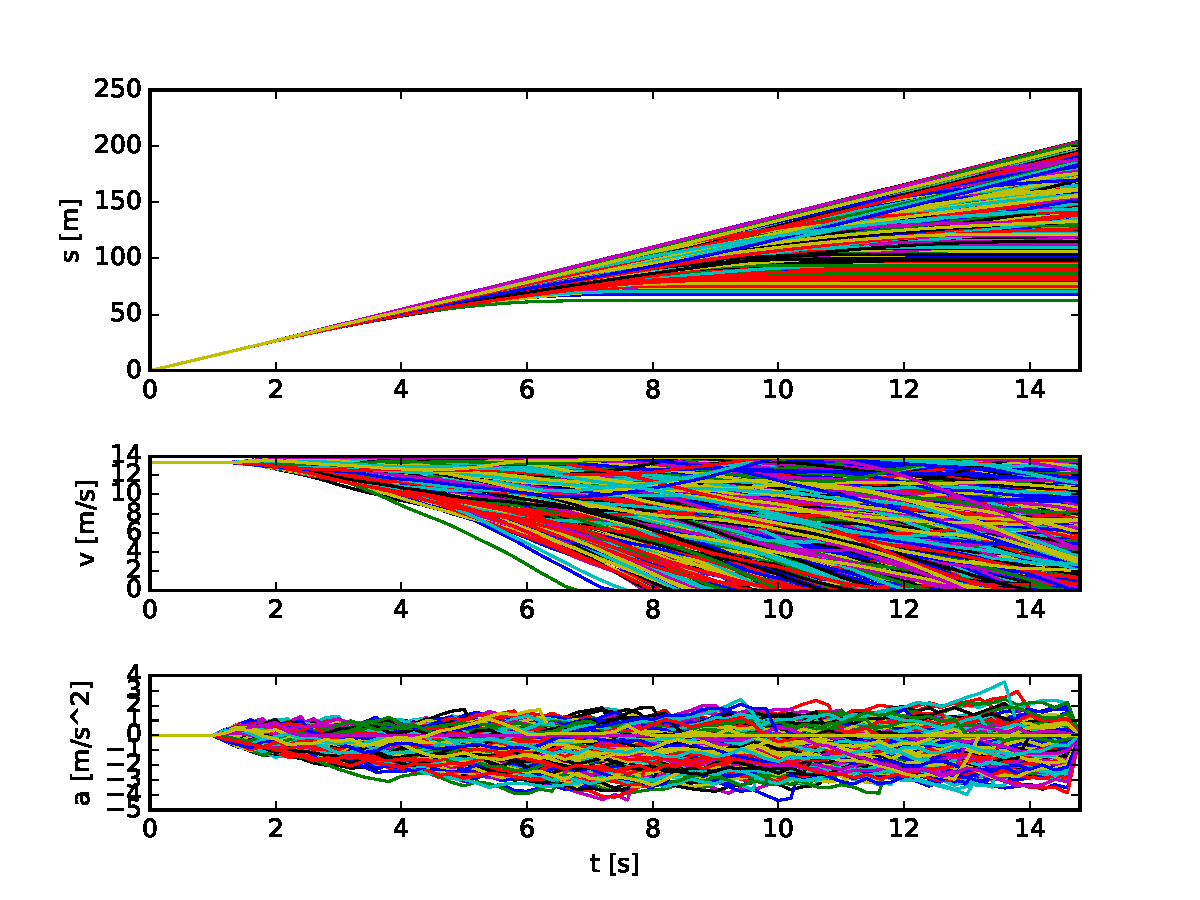
\includegraphics[width = 0.7 \textwidth ]{Geschwindigkeitsprofile.pdf}
    \caption[Erzeugung von Geschwindigkeitsprofilen]{Darstellung von 1000 zuf\"allig ermittelten Geschwindigkeitsprofilen. In der ersten Sekunde stimmen alle Geschwindigkeitsprofile \"uberein, da hier die Trajektorie aus dem vorausgegangen Planungsschritt \"ubernommen wird.}
    \label{fig:Geschwindgkeitsprofile}
\end{figure}


\subsection{Berechnung der normalisierten Sicherheitsabst\"ande}
Wie in Kapitel~\ref{sec:LCKostfunc} beschrieben werden zur Berechnung des Kostentermes \gls{symb:G_sd} normalisierte Sicherheitsabst\"ande \gls{symb:d_normal} berechnet.
Die Berechnung der normalisierten Sicherheitsabst\"ande findet an den diskreten Zeitschritten statt.
Es wurde drauf verzichtet, diese Abst\"ande ausschlie{\ss}lich f\"ur das Fahrzeug, das sich direkt vor dem Ego"=Fahrzeug auf dem selben Fahrstreifen befindet, zu berechnen.
Vielmehr wurden bei der Berechnung alle Fahrzeuge der Simulation betrachtet.
Damit ist gew\"ahrleistet, dass die fahrstreifenbasierte Pr\"adiktion durch eine komplexere Pr\"adiktion ausgetauscht werden kann, ohne dass die Berechnung der normalisierten Sicherheitsabst\"ande neu implementiert werden muss.
Eine komplexere Pr\"adiktion k\"onnte auch Fahrstreifenwechselintensionen von anderen Fahrzeugen ber\"ucksichtigen.

Um den Rechenaufwand nicht unn\"otig zu steigern wurde eine Filterfunktion eingebaut.
Diese schlie{\ss}t Fahrzeuge die sich an einem diskreten Zeitpunkt hinter dem betrachteten Fahrzeug oder weit vor diesem befinden von der Ber\"ucksichtigung aus.


\subsection{Anpassung des \gls{idm}}
Die in Kapitel~\ref{sec:IDMpred} vorgestellte Formel des \gls{idm} zur Berechnung eines Geschwindigkeitsprofiles f\"ur ein Fahrzeug in Folgefahrt sorgt f\"ur ein nicht zufriedenstellendes Fahrverhalten.
Es wurden deshalb folgende Anpassungen vorgenommen:

\begin{itemize}


\item \textit{Begrenzung des Rucks}: Ein hoher Ruck wird von Fahrzeuginsassen als besonders unangenehm empfunden. 
Bei der Berechnung der Beschleunigungswerte werden diese deshalb so begrenzt werden, dass sowohl ein negativer als auch positiver Grenzwert (\(j_\mathrm{min}\) und \(j_\mathrm{max}\)) des Rucks nicht \"uberschritten wird.

\item \textit{Ausschlu{\ss} von negativen Geschwindigkeiten}: Es wird davon ausgegangen, dass bei einem normalen Fahrstreifenwechselman\"over keines der beteiligten Fahrzeuge r\"uckw\"arts f\"ahrt.
Deshalb wird bei der Berechnung der Beschleunigung eine minimal zul\"assige Beschleunigung berechnet, bei der das Fahrzeug zum Stillstand kommen w\"urde.

\item \textit{Abschnittsweise Unterdr\"uckung des interaktiven Terms}: Der interaktive Term sorgt daf\"ur, dass selbst bei gro{\ss}em Abstand zum Vorderfahrzeug die optimale Geschwindigkeit bis zum n\"achsten Abtastzeitpunkt nicht konstant gehalten wird.
Der interaktive Term wird deshalb bei gro{\ss}em Abstand zum Vorderfahrzeug unterdr\"uckt.
Erst wenn der Abstand der Fahrzeuge \( s_\alpha < 1.3 s^*\) ist wird der interaktive Term zur Berechnung der Beschleunigung ber\"ucksichtigt.
Der Term \(s^*\) ist der im \gls{idm} berechnete Wunschabstand des Folgefahrzeuges zum vorderen Fahrzeug (vgl. Kapitel~\ref{sec:IDMpred}).

\end{itemize}



\section{Auswertung}

In diesem Abschnitt werden die Simulationsergebnisse vorgestellt und diskutiert.
Eine eindeutige Aussage \"uber die Qualit\"at eines Trajektorienplanungsansatzes zu Treffen ist nur sehr schwer m\"oglich.
Die Bewertung anhand eines Kostenfunktionals h\"angt stark von dem gew\"ahlten Kostenfunktional ab.
Dieses Kostenfunktional soll daf\"ur sorgen, dass es zu keiner Kollision mit Hindernissen oder anderen Verkehrsteilnehmern kommt.
Weiter noch soll es zu einer Trajektorie f\"uhren die von den Insassen als m\"oglichst angenehm empfunden wird.
Dieses Empfinden h\"angt stark von der betreffenden Person ab.
Entsprechend muss das Kostenfunktional, um die tats\"achlich optimale Trajektorie zu ermitteln, auf die Person angepasst sein.
Eine konkrete Aussage \"uber die Qualit\"at einer Trajektorie anhand der Kosten ist dementsprechend immer nur f\"ur eine bestimmt Person zul\"assig.

Es lassen sich jedoch qualitative Aussagen treffen.
So sollten in der Regel hohe R\"ucke und Beschleunigungen vermieden werden.
Zus\"atzlich sollte das Fahrzeug mit einer Geschwindigkeit fahren die m\"oglichst nah an einer gew\"unschten optimalen Geschwindigkeit liegt und Abst\"ande zu anderen Fahrzeugen sollten nicht zu gering sein.
In der Regel ist es nicht m\"oglich alle Aspekte komplett zu erf\"ullen.
Die einzelnen Kostenterme spiegeln wider wie stark die Trajektorie von den Optimalwerten abweicht.

Eine weitere Schwierigkeit besteht darin, dass bei diesem Ansatz ein Trajektorienset gefunden werden soll, bei dem die Interaktion mit anderen Fahrzeugen ber\"ucksichtigt wird.
Daf\"ur muss pr\"adiziert werden, wie andere Fahrzeuge auf das eigene Fahrverhalten reagieren werden.
Die Reaktion der Fahrzeuge Testdaten zu entnehmen ist kaum m\"oglich.
Zum einen m\"ussten dadurch auch sicherheitskritische Situationen getestet werden.
Zum anderen ist die Reaktion sehr personenspezifisch und spiegelt nur eine von vielen m\"oglichen Reaktionen wieder.
Laut Naumann et al. \cite{Naumann2018} gibt es drei M\"oglichkeiten warum ein Fahrzeug von der vorhergesagten Trajektorie abweicht:
\begin{itemize}
\item Das Kostenfunktional oder das Ziel des betreffenden Fahrzeuges wurde falsch eingesch\"atzt.
\item Das Fahrzeug hat das Kostenfunktional des Ego"=Fahrzeuges falsch eingesch\"atzt.
\item Das Fahrzeug verh\"alt sich nicht entsprechend der angenommenen Verhaltenspolitik.
\end{itemize}
F\"ur eine pr\"azise Pr\"adiktion m\"usste also das Kostenfunktional des interagierenden Fahrzeuges bekannt sein.
Dies ist in der Regel nicht der Fall.
Ist es bekannt, ist dennoch nicht sichergestellt, ob sich das Fahrzeug dementsprechend verhalten wird.
 
Bei der Evaluierung des Ansatzes soll deshalb zuerst davon ausgegangen werden, dass andere Fahrzeuge sich entsprechend der vom Ansatz generierten Bewegungspr\"adiktion verhalten.
Es werden zun\"achst die Ergebnisse eines einzelnen Planungsschrittes betrachte.
Anschlie{\ss}end wird der Ansatz bei einer fortlaufenden Neuplanung untersucht.
Dabei soll zuerst von einem kooperativen Verhalten der anderen Verkehrsteilnehmer ausgegangen werden.
Anschlie{\ss}end wird untersucht wie das Ego"=Fahrzeug durch den vorgestellten Ansatz auf ein egoisitisches Verhalten der anderen Verkehrsteilnehmer reagiert.

Zur Beurteilung der sich ergebenden Trajektoriensets k\"onnen folgende Fragen genutzt werden:
\begin{itemize}
\item Wird ein kooperatives Verhalten der Verkehrsteilnehmer widergespiegelt?
\item Werden kollisionsfreie Trajektorien generiert?
\item Werden Sicherheitsabst\"ande eingehalten?
\item Wie stark sind die Abweichungen der einzelnen Fahrzeuge von den angenommenen Wunschgeschwindigkeiten?
\item Wie hoch sind die Beschleunigungen der betrachteten Fahrzeuge?
\end{itemize}


In den Simulationen wurde f\"ur jedes Fahrzeug das gleich Kostenfunktional angenommen.
Die entsprechenden Parameter sind in Tabelle~\ref{tab:Kostfunc} im Anhang gegeben. 
In einzelnen F\"allen weicht das Kostenfunktional des Ego"=Fahrzeuges von diesen Parametern ab.
Ist dies der Fall wird darauf hingewiesen und die Abweichung begr\"undet.

Die Fahrzeuge auf dem Zielfahrstreifen werden zum Zweck einer eindeutigen Beschreibung durchnummeriert.
Das vorderste Fahrzeug auf dem Zielfahrstreifen wird als Fahrzeug 2 bezeichnet.
Die Fahrzeug dahinter werden aufsteigend bis zum hintersten Fahrzeug durchnummeriert.

\subsection{Einzelner Planungsschritt}
\label{sec:einzelPlanungsschritt}
Es sollen zun\"achst die Ergebnisse eines einzelnen Planungsschrittes betrachtet werden.
Die Ergebnisse zeigen jeweils die erzeugte Trajektorie des Ego"=Fahrzeuges und die kooperative Bewegungspr\"adiktion der anderen Fahrzeuge.
Nur f\"ur den Fall, dass sich alle Fahrzeuge entsprechend diesem Trajektorienset verhalten entspricht dies auch dem letztentlich gefahrenen Trajektorienset.
Dies ist in der Regel nicht der Fall.
Es werden deshalb sowohl eine Neuplanung als auch Sicherheits\"uberpr\"ufungen notwendig.
Trotzdem ist es sinnvoll zun\"achst die Ergebnisse eines einzelnen Planungsschrittes zu analysieren um grundlegende Aussagen \"uber den Planungsansatz treffen zu k\"onnen.
Der in dieser Arbeit vorgestellte Ansatz wurde in verschiedenen Szenarien getestet.
Die verschiedenen Szenarien und repr\"asentativen Simulationsergebnisse der Szenarien werden im Folgenden vorgestellt.


\minisec{Zwei Fahrzeuge auf dem Zielfahrstreifen}
Im ersten Szenario befinden sich zwei Fahrzeuge auf dem Zielfahrstreifen.
Das Ego"=Fahrzeug befindet sich auf dem Fahrstreifen rechts neben den beiden Fahrzeugen und in lateraler Richtung zwischen den beiden Fahrzeugen.
Der Abstand zwischen den Fahrzeugen 2 und 3 ist anf\"anglich so gro{\ss}, dass kein weiteres Fahrzeug zwischen ihnen auf den Zielfahrstreifen auffahren kann, ohne dass Sicherheitsabst\"ande deutlich unterschritten werden.
Die Anfangsgeschwindigkeit der Fahrzeuge entspricht ihrer Optimalgeschwindigkeit und ist so gew\"ahlt, dass das Ego"=Fahrzeug bei einer egoistischen Planung zwischen den Fahrzeugen auf den Zielfahrstreifen auffahren w\"urde.
Eine sichere Fahrstreifenwechseltrajektorie kann deshalb nur gefunden werden, wenn mindestens eines der Fahrzeuge von seiner Optimalgeschwindigkeit abweicht.
Die Ausgangsposition ist in Abbildung~\ref{fig:two_veh_scene} dargestellt.
Die Startzust\"ande der Fahrzeuge sind in Tabelle~\ref{tab:StartS1} gegeben.
 
\begin{figure}[!htbp]
    \centering
    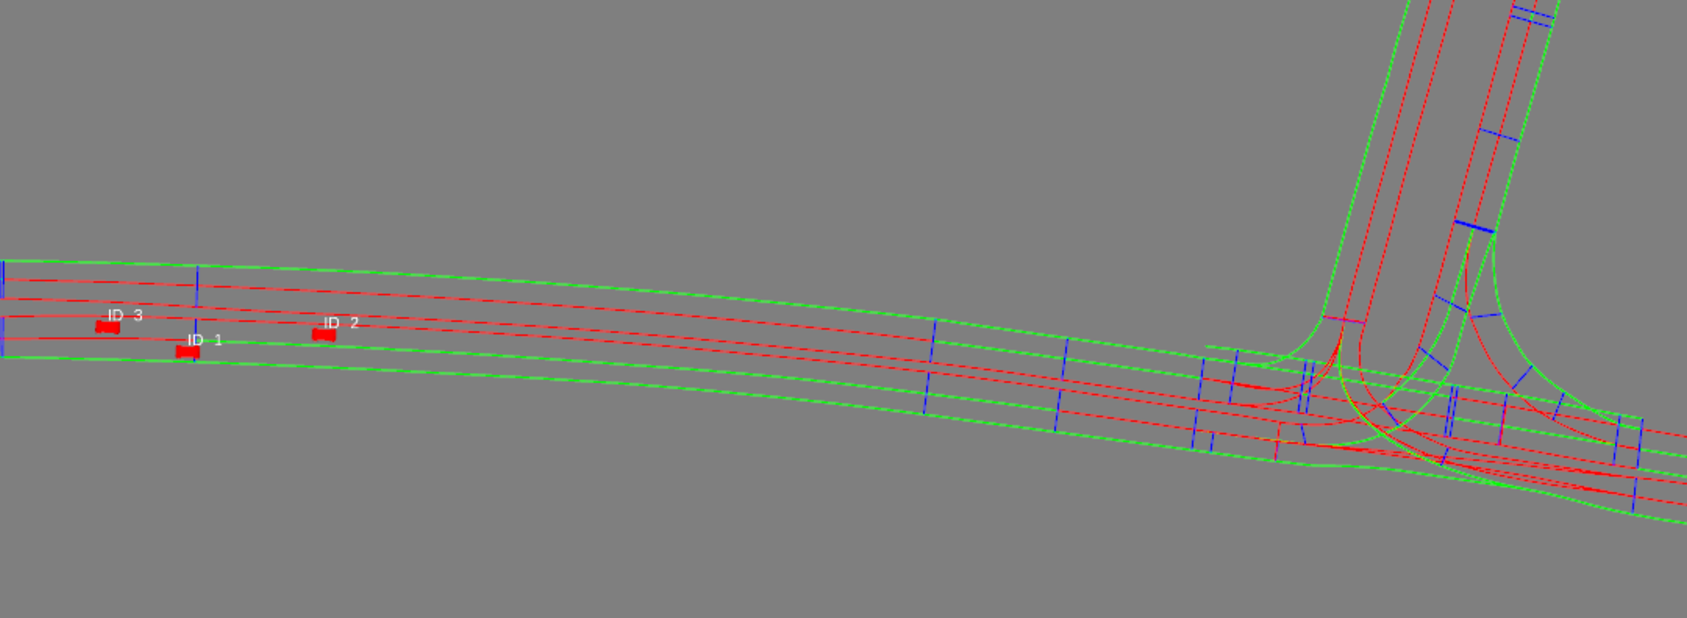
\includegraphics[width = 0.8 \textwidth ]{two_veh_sce.pdf}
    \caption[Szenario 1]{Ausgangsposition der Fahrzeuge im ersten Szenario}
    \label{fig:two_veh_scene} 
\end{figure}

\sisetup{round-mode = places, round-precision = 2, scientific-notation = fixed, fixed-exponent = 0}
\begin{table}[!htbp]
    \centering
    \begin{tabular}{crSSSS}
        \hline
        & & {\gls{symb:a_start}  [m/s\textasciicircum 2]} & {\gls{symb:v_start} [km/h]} & {\gls{symb:v_opt} [km/h]} & {Abstand zu   \gls{symb:s_cmax} [m]} \\%
        \hline
        & Ego"=Fahrzeug & 00.00e+00 & 48.00e+00 & 48.00e+00 & 108.65e+00\\
        & Fahrzeug 2 & 00.00e+00 & 48.00e+00 & 48.00e+00 & 86.74e+00\\
        & Fahrzeug 3 & 00.00e+00 & 48.00e+00 & 48.00e+00 & 121.71e+00\\
         \hline
    \end{tabular}
    \caption[Startzust\"ande Szenario 1]{Startzust\"ande der Fahrzeuge im ersten Szenario.
    }\label{tab:StartS1}
\end{table}

Das Ergebnis eines einzelnen Planungsschrittes ist in Abbildung~\ref{zweiFahrzeugeKoop} dargestellt.
Das Ego"=Fahrzeug ordnet sich zwischen den beiden Fahrzeugen auf dem Zielfahrstreifen ein.
Beide Fahrzeuge auf dem Zielfahrstreifen zeigen ein kooperatives Verhalten.
Das vordere Fahrzeug (Fahrzeug 2) f\"ahrt bereits sehr nahe an der maximalen Geschwindigkeit.
Deshalb ist das kooperative Verhalten nicht stark ausgepr\"agt.
Es ist lediglich ein leichtes Erh\"ohen der Geschwindigkeit zu erkennen.
Das Ego"=Fahrzeug senkt seine Geschwindigkeit bis zum Fahrstreifenwechsel leicht ab um den entsprechenden Sicherheitsabstand zum vorderen Fahrzeug beim Auffahren auf den Zielfahrstreifen einzuhalten.
Anschlie{\ss}end beschleunigt es um sich wieder seiner Optimalgeschwindigkeit anzun\"ahern.
Beim hinteren Fahrzeug auf dem Zielfahrstreifen (Fahrzeug 3) ist eindeutiges kooperatives Verhalten zu erkennen.
Es weicht von seiner Optimalgeschwindigkeit ab um dem Ego"=Fahrzeug das Auffahren auf den Zielfahrstreifen zu erleichtern.
Der laterale Abstand zwischen den beiden Fahrzeugen w\"achst ab dem Zeitpunkt, ab dem die Fahrstreifenwechselintension erkannt wird, bis zum Fahrstreifenwechsel kontinuierlich an.
Sobald sich das Ego"=Fahrzeug auf dem Zielfahrstreifen befindet geht Fahrzeug 3 in die Folgefahrt \"uber und f\"angt an seine Geschwindigkeit wieder zu erh\"ohen.
Gegen Ende des Planungshorizontes haben sich alle Fahrzeuge wieder ihrer Optimalgeschwindigkeit angen\"ahert und es haben sich nahezu gleichm\"a{\ss}ige Abst\"ande zwischen den Fahrzeugen gebildet.

Zum Vergleich ist in Abbildung~\ref{zweiFahrzeugeEgo} das Ergebnis dargestellt, wenn von einem egoistischen Verhalten der Fahrzeuge auf dem Zielfahrstreifen ausgegangen wird.
Hierzu wurden zuf\"allige Trajektorien des Ego"=Fahrzeuges generiert.
Die Fahrzeuge auf dem Zielfahrstreifen behalten ihre Geschwindigkeit bei.
Ihre Trajektorie ist somit vorgegeben.
Anschlie{\ss}end wird jede generierte Trajektorie des Ego"=Fahrzeuges mit den vorgegebenen Trajektorien der Fahrzeuge auf dem Zielfahrstreifen kombiniert und das sich ergebende Trajektorienset anhand des Kostenfunktionals bewertet.
Zur Generierung der zuf\"alligen Trajektorien des Ego"=Fahrzeuges wurde der selbe Algorithmus verwendet wie in der kooperativen Simulation in der von einem kooperativen Verhalten der anderen Fahrzeuge ausgegangen wird. 
Die Bewertung der Trajektorie fand mit dem gleiche Kostenfunktional.

Bei einem egoistischen Verhalten der Fahrzeuge auf dem Zielfahrstreifen ist das Ego"=Fahrzeug gezwungen diese zuerst passieren zu lassen.
Dazu muss es deutlich von seiner Optimalgeschwindigkeit abweichen.
Die minimale Geschwindigkeit des Ego"=Fahrzeuges ist deutlich geringer als bei der Annahme eines kooperativen Verhaltens.
Erst wenn die Fahrzeuge auf dem Zielfahrstreifen vorbeigefahren sind kann das Ego"=Fahrzeug wieder beschleunigen und auf den Zielfahrstreifen auffahren.

Die einzelnen Kostenterme der beiden Szenarien sind in Tabelle~\ref{tab:Kostenvergleich} gegen\"ubergestellt.
Ein Vergleich der Kostenterme spiegelt die gemachten Beobachtungen wieder.
Der Geschwindigkeitsterm \gls{symb:G_v} des Ego"=Fahrzeuges konnten durch ein kooperatives Verhalten der Fahrzeuge auf dem Zielfahrstreifen deutlich herabgesetzt werden.
Auch die Kostenterme \gls{symb:G_a} und \gls{symb:G_sd}  fallen geringer aus.
Im Gegenzug kommen bei den Gesamtkosten Kosten f\"ur das kooperative Fahrzeug hinzu.
Doch auch hier spiegelt der Geschwindigkeitsterm wider, dass das Fahrzeug wesentlich weniger von seiner Optimalgeschwindigkeit abweichen muss als das Ego-Fahrzeug bei einem unkooperativen Fahrstreifenwechsel.
Insgesamt konnten die Kosten basierend auf dem verwendeten Kostenfunktional um \(47.43\%\) gesenkt werden.

\begin{figure}[!htbp]
    \centering
    \subfigure[Kooperativ ]{
        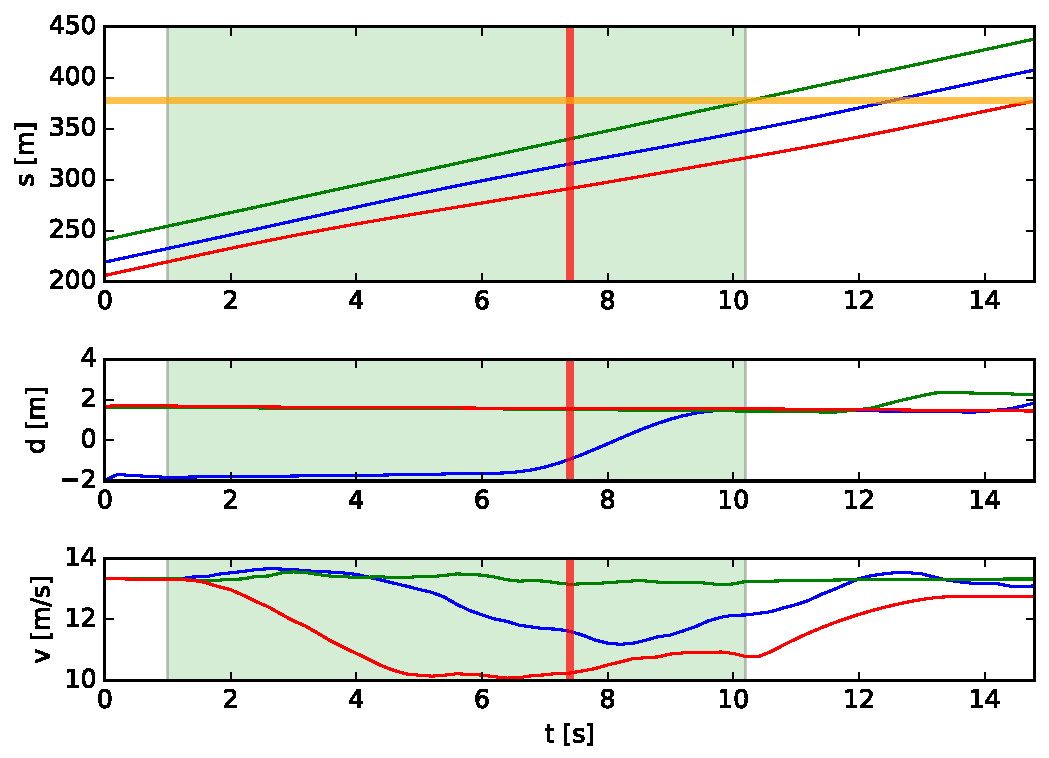
\includegraphics[width =  0.8 \textwidth]{two_veh_result.pdf}
        \label{zweiFahrzeugeKoop}
    }
    \subfigure[Unkooperative]{
        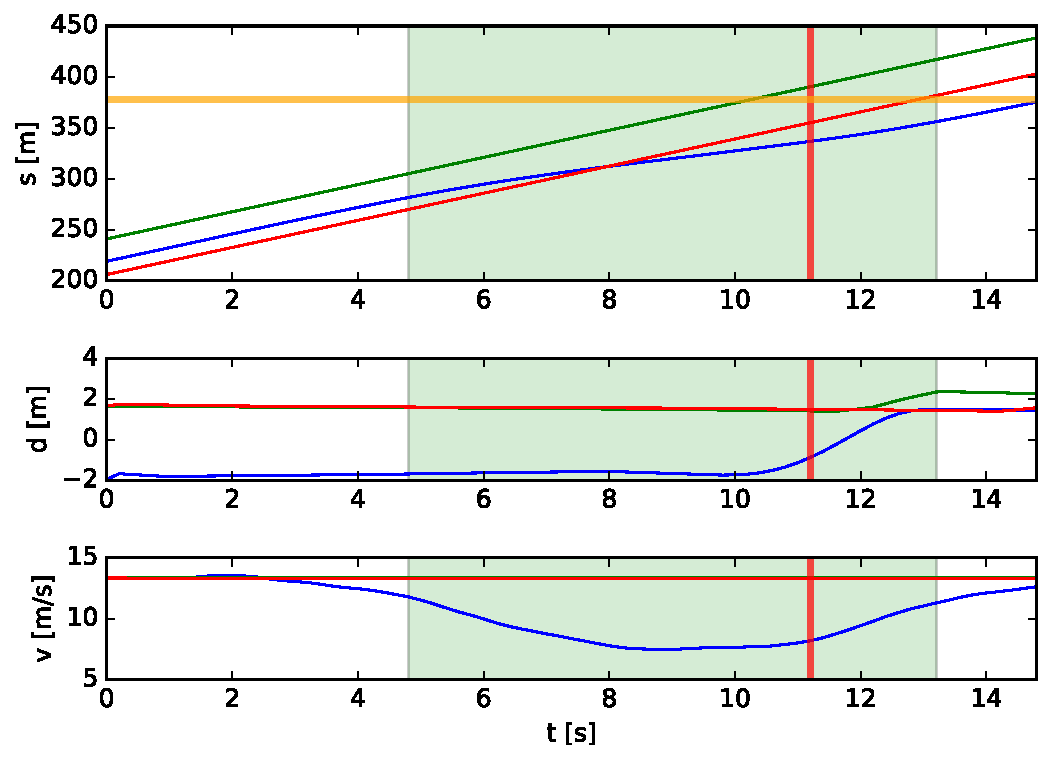
\includegraphics[width = 0.8  \textwidth]{two_veh_ego_result.pdf}
        \label{zweiFahrzeugeEgo}
    }
    \caption[Fahrstreifenwechsel Vergleich]{Vergleich von einem kooperativen und einem unkooperativen Fahrstreifenwechsel. 
    Das Ego"=Fahrzeug ist durch die blaue Line gekennzeichnet die restlichen Fahrzeuge befinden sich auf dem Zielfahrstreifen.
    Der Zeitbereich von \gls{symb:t_coop,start} bis \gls{symb:t_coop,end} ist gr\"un hinterlegt. Die vertikale rote Line kennzeichnet den Zeitpunkt des Fahrstreifenwechsels \gls{symb:t_lc}. Die orange horizontale Line kennzeichnet bis zu welcher Wegstrecke \gls{symb:s_cmax} der Fahrstreifenwechsel beendet sein muss.
    (Am Ende des Planushorizonts ist ein Anstieg von \gls{symb:d_r} zu sehen nach dem der Fahrstreifenwechsel durchgef\"uhrt wurde. Dies liegt daran, das hier der Pfad des Zielfahrstreifens st\"arker von der Referenzkurve abweicht. Die Fahrzeuge befinden sich noch immer auf dem Zielfahrstreifen)}
    \label{fig:Vergleich}
\end{figure}


\sisetup{round-mode = places, round-precision = 2, scientific-notation = fixed, fixed-exponent = 0}
\begin{table}[!htbp]
    \centering
    \begin{tabular}{crSSSSS|S}
        \hline
        & & \textbf{\gls{symb:G_a}} & \textbf{\gls{symb:G_v}} & \textbf{\gls{symb:G_sd}} & \textbf{\gls{symb:G_lc}} & \textbf{\gls{symb:G_lcend}} & {Fahrzeugkosten}\\%
        \hline
        & Ego"=Fahrzeug & 15.13e+00 & 8.30e+00 & 0.00e+00 & 0.0e+00 & x & 23.43e+00\\
        & Fahrzeug 2 & 1.76e+00 & 0.11e+00 & 0.0e+00 & 0.0e+00 & 0.19e+00 & 2.06e+00\\
        & Fahrzeug 3 & 21.96e+00 & 37.37e+00 & 0.09e+00 & 0.0e+00 & 10.46e+00 & 69.88e+00\\
        & Multi-Agenten & 38.85e+0 & 45.78e+00 & 0.09e+00 & 0.0e+00 & 10.65e+00 & 95.37e+00\\
        \hline
        &  Egoistische Pr\"adiktion& 61.09e+00 & 115.40e+00 & 4.91e+00 & 0.00e+00 & x & 181.40e+00\\
         \hline
    \end{tabular}
    \caption[Kostenvergleich]{Vergleich der Kosten eines kooperativen Fahrstreifenwechsels ermittelt durch eine Multi-Agenten-Optimierung und eines unkooperativen Fahrstreifenwechsels.
    }\label{tab:Kostenvergleich}
\end{table}



\minisec{Vier Fahrzeuge auf dem Zielfahrstreifen}
Im ersten Szenario konnte gezeigt werden, dass durch den vorgestellten Ansatz ein kooperatives Verhalten der Fahrzeuge auf dem Zielfahrstreifen widergespiegelt werden kann.
Im Vergleich dazu ist das Ego"=Fahrzeug bei einem egoistischen Verhalten der anderen Verkehrsteilnehmer gezwungen deutlich st\"arker von seiner Optimalgeschwindigkeit abzuweichen.
Es kann den Fahrstreifenwelchsel jedoch auch ohne kooperatives Verhalten der anderen Verkehrsteilnehmer durchf\"uhren, ohne dabei auf dem aktuellen Fahrstreifen anzuhalten.
Im Folgenden soll nun \"ahnliche Szenarien untersucht werden, wobei sich jedoch vier Fahrzeuge auf dem Fahrstreifen befinden.
Damit soll eine dicht befahrene Stra{\ss}e dargestellt werden.
Der Abstand zwischen den Fahrzeugen auf dem Zielfahrstreifen ist anf\"anglich wieder so gew\"ahlt, dass die L\"ucken nicht gro{\ss} genug f\"ur einen sicheren Fahrstreifenwechsel sind.
Die Ausgangspositionen der Fahrzeuge sind in Abbildung~\ref{fig:four_veh_scene} dargestellt.
Zuerst wird in Szenario 2.1 \"ahnlich zum ersten Szenario angenommen, dass das Ego"=Fahrzeug die gleiche Geschwindigkeit wie die Fahrzeuge auf dem Zielfahrstreifen hat.
In den Szenarien 2.2, 2.3 und 2.4 wird dann die Geschwindigkeit des Ego-Fahrzeuges variiert.
Es wird angenommen, dass die niedrigere Anfangsgeschwindigkeit nicht durch Interaktion mit anderen Fahrzeugen verursacht wurde.
Deshalb ist nicht davon auszugehen das die Anfangsgeschwindigkeit bereits im diskomfortablen Bereich liegt.
Das Kostenfunktional des Ego"=Fahrzeuges wird bei den entsprechenden Szenarien deshalb so angepasst, dass der unkomfortable Bereich f\"ur negative Abweichungen von der Optimalgeschwindigkeit unter der Anfangsgeschwindigkeit des Ego"=Fahrzeuges beginnt.
Die Startzust\"ande der Fahrzeuge auf dem Zielfahrstreifen bleiben in allen Szenarien unver\"andert.
Die Anfangszust\"ande der Fahrzeuge f\"ur die verschiedenen Szenarien sind in Tabelle~\ref{tab:StartS2} gegeben.

\begin{figure}[!htbp]
    \centering
    \includegraphics[width = 0.8 \textwidth ]{four_veh_sce.pdf}
    \caption[Szenario 2]{Ausgangsposition der Fahrzeuge in den Szenarien 2.1, 2.2, 2.3, 2.4}
    \label{fig:four_veh_scene} 
\end{figure}


\sisetup{round-mode = places, round-precision = 2, scientific-notation = fixed, fixed-exponent = 0}
\begin{table}[!htbp]
    \centering
    \begin{tabular}{crSSSS}
        \hline
        & & {\gls{symb:a_start}  [m/s\textasciicircum 2]} & {\gls{symb:v_start} [km/h]} & {\gls{symb:v_opt} [km/h]} & {Abstand zu   \gls{symb:s_cmax} [m]} \\%
        \hline
        & Fahrzeug 2 & 00.00e+00 & 48.00e+00 & 48.00e+00 & 86.74e+00\\
        & Fahrzeug 3 & 00.00e+00 & 48.00e+00 & 48.00e+00 & 121.71e+00\\
        & Fahrzeug 4 & 00.00e+00 & 48.00e+00 & 48.00e+00 & 156.65e+00\\
        & Fahrzeug 5 & 00.00e+00 & 48.00e+00 & 48.00e+00 & 191.69e+00\\
         \hline
         & Ego"=F. Sze. 2.1 & 00.00e+00 & 48.00e+00 & 48.00e+00 & 108.65e+00\\
         & Ego"=F. Sze. 2.2 & 00.00e+00 & 40.00e+00 & 48.00e+00 & 108.65e+00\\
         & Ego"=F. Sze. 2.3 & 00.00e+00 & 30.00e+00 & 48.00e+00 & 108.65e+00\\
         & Ego"=F. Sze. 2.4 & 00.00e+00 & 25.00e+00 & 48.00e+00 & 108.65e+00\\
          \hline
    \end{tabular}
    \caption[Startzust\"ande Szenarien 2]{Startzust\"ande der Fahrzeuge f\"ur die Szenarien mit vier Fahrzeugen auf dem Zielfahrstreifen.
    }\label{tab:StartS2}
\end{table}

Im Vergleich zum ersten Szenario werden in den folgenden Szenarien zwei weitere Fahrzeuge in der Simulation in Betracht gezogen.
Die Anzahl der potentiellen kooperativen Partner wurde somit verdoppelt.
Die Simulationen fanden auf dem gleichen Rechner und unter der Nutzung gleich vieler Kerne statt.
Die Rechenzeit ist im Vergleich um lediglich 63\% und damit weniger als linear mit der Anzahl der Fahrzeuge angestiegen.

Die Simulationsergebnisse von Szenario 2.1 sind in Abbildung~\ref{fig:VierFahrzeuge} dargestellt.
Es zeigt sich ein \"ahnliches Verhalten wie im ersten Szenario.
Das Ego"=Fahrzeug f\"ahrt in die L\"ucke zwischen den Fahrzeugen 2 und 3 ein.
Das vorderste Fahrzeug auf dem Zielfahrstreifen (Fahrzeug 2) bleibt von dem Fahrstreifenwechselman\"over weitesgehend unbeeinflusst.
Das zweite Fahrzeug auf dem Zielfahrstreifen (Fahrzeug 3) senkt seine Geschwindigkeit ab um die L\"ucke f\"ur den Fahrstreifenwechsel zu vergr\"o{\ss}ern.
Nach Beendigung des Fahrstreifenwechsels beschleunigt es, um sich seiner Optimalgeschwindigkeit anzun\"ahern.
Die zwei hinteren Fahrzeuge (4 und 5) verhalten sich entsprechend des \gls{idm}.
Sie bremsen zuerst ab, um den Sicherheitsabstand zum vorausfahrenden Fahrzeug einzuhalten und beschleunigen, sobald das vorausfahrende Fahrzeuge die Geschwindigkeit erh\"oht und somit die L\"ucke vergr\"o{\ss}ert wird.
Am Ende des Planungshorizonts haben sich zwischen den Fahrzeugen wieder nahezu gleichm\"a{\ss}ige Abst\"ande gebildet.


\begin{figure}[!htbp]
    \centering
    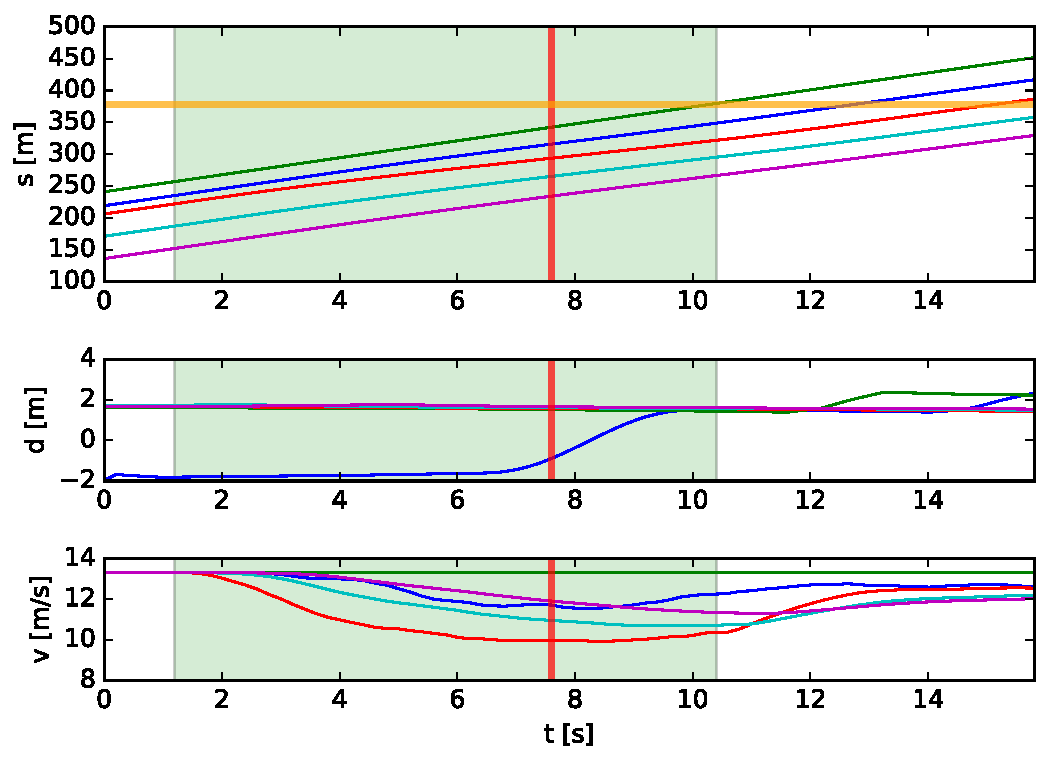
\includegraphics[width = 0.85 \textwidth ]{four_veh_results.pdf}
    \caption[Ergebnisse Szenario 2.1]{Kooperativer Fahrstreifenwechsel bei vier Fahrzeugen auf dem Zielfahrstreifen. F\"ur die Legende sei auf Abbildung~\ref{zweiFahrzeugeEgo} verwiesen.}
    \label{fig:VierFahrzeuge} 
\end{figure}


In den Abbildung~\ref{fig:VerschiedeneGeschwindigkeiten} sind die Simulationsergebnisse f\"ur verschiedene Anfangsgeschwindigkeiten des Ego"=Fahrzeuges zu sehen.
In Abbildung~\ref{40kmh} ist zu sehen, dass das Ego-Fahrzeug bei einer Anfangsgeschwindigkeit von 40 km/h die gleiche L\"ucke w\"ahlt wie in den zuvor betrachteten Szenarien.
In der ersten Sekunde folgt das Ego"=Fahrzeug noch der Trajektorie aus dem angenommenen vorausgegangen Zeitschritt.
Anschlie{\ss}end beschleunigt es und passt damit seine Geschwindigkeit den Fahrzeugen auf dem Zielfahrstreifen an.
Das zweite Fahrzeug auf dem Zielfahrstreifen (Fahrzeug 3) zeigt erneut ein kooperatives Verhalten und verringert seine Geschwindigkeit.
Damit wird der longitudinale Abstand zwischen den Fahrzeugen bis zum Fahrstreifenwechsel vergr\"o{\ss}ert, sodass sich eine L\"ucke bildet die gro{\ss} genug f\"ur einen sicheren Fahrstreifenwechsel des Ego"=Fahrzeuges ist.

In Szenario 2.3 startet das Ego"=Fahrzeug mit 30 km/h (siehe Abbildung~\ref{30kmh}).
Es besteht nicht mehr auf die L\"ucke zwischen den Fahrzeugen 2 und 3.
Wie in Szenario 2.2 beschleunigt das Ego"=Fahrzeug, um sich der Geschwindigkeit auf dem Zielfahrstreifen anzupassen.
Es beh\"alt jedoch eine deutlich geringere Geschwindigkeit bei bis das Fahrzeug 3 passiert ist.
Anschlie{\ss}end beschleunigt es erneut um sich der Optimalgeschwindigkeit anzun\"ahern.
In diesem Fall zeigt Fahrzeug 4 ein kooperatives Verhalten, indem es seine Geschwindigkeit verringert.
In Abbildung~\ref{25kmh} ist das Verhalten des Ego"=Fahrzeuges bei einer Startgeschwindigkeit von 25 km/h zu sehen.
Da sich hinter den vier Fahrzeugen auf dem Zielfahrstreifen eine L\"ucke ergibt, die gro{\ss} genug ist, beh\"alt das Ego"=Fahrzeug seine vergleichsweise niedrige Geschwindigkeit bei und l\"asst die Fahrzeuge auf dem Zielfahrstreifen passieren.
Es zwingt dadurch keines der Fahrzeuge auf dem Zielfahrstreifen dazu, seine Geschwindigkeit drastisch anzupassen.
Der Fahrstreifenwechsel findet ohne kooperatives Verhalten der Fahrzeuge auf dem Zielfahrstreifen statt.

Die Szenarien zeigen, dass der Ansatz durch die Annahme eines kooperativen Verhaltens der Fahrzeuge auf dem Zielfahrstreifen auch einen Fahrstreifenwechsel bei dichtem Verkehr erlaubt.
Ist die anf\"angliche Geschwindigkeit des Ego-Fahrzeuges niedriger als die der Fahrzeuge auf dem Zielfahrstreifen beschleunigt es zuerst, um seine Geschwindigkeit anzupassen und ordnet sich dann im Zielfahrstreifen ein.
Dieses Verhalten entspricht dem Verhalten, das auf einer Beschleunigungsspur gefordert ist.
Es kann jedoch auch gezeigt werden, dass das Ego"=Fahrzeug nicht auf ein kooperatives Verhalten der Fahrzeuge auf dem Zielfahrstreifen besteht, wodurch es selbst ein egoistisches Verhalten zeigen w\"urde.
Sind die eigenen Vorteile im Vergleich zu den Nachteilen der kooperativen Fahrzeuge nicht gro{\ss} genug wird nicht von einem kooperativen Verhalten der anderen Fahrzeuge ausgegangen.


\begin{figure}[!htbp]
    \centering
    \label{fig:VerschiedeneGeschwindigkeiten}
    \subfigure[40 km/h ]{
        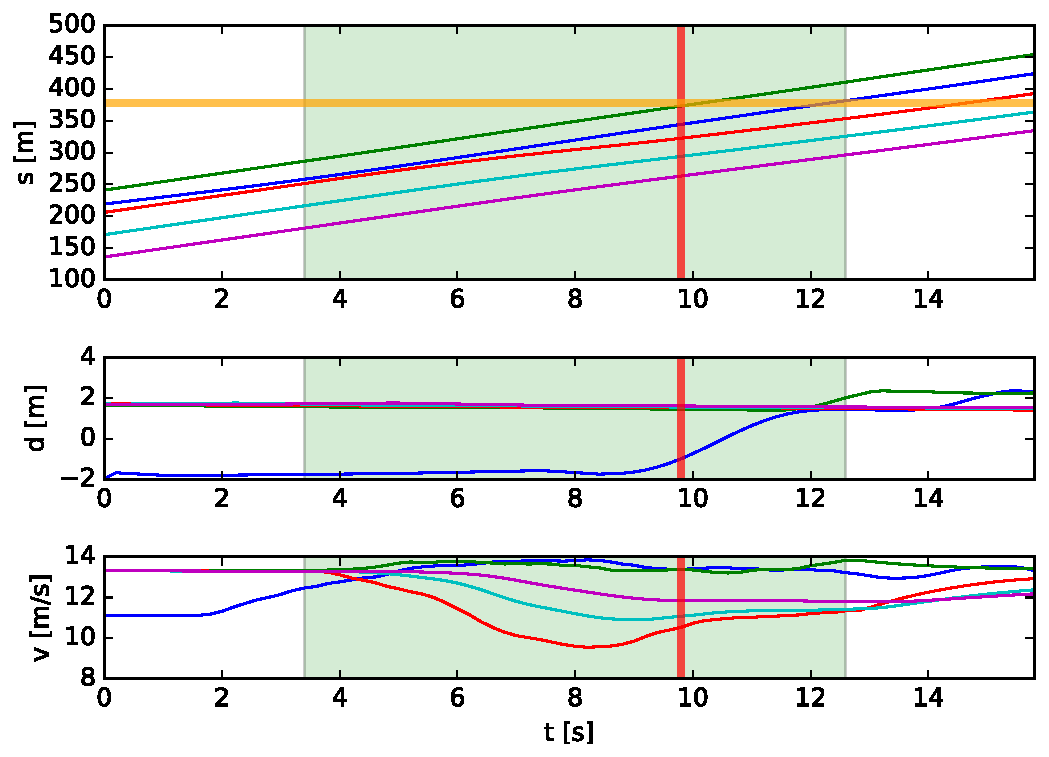
\includegraphics[width =  0.63 \textwidth]{40_kmh.pdf}
        \label{40kmh}
    }
    \subfigure[30 km/h]{
        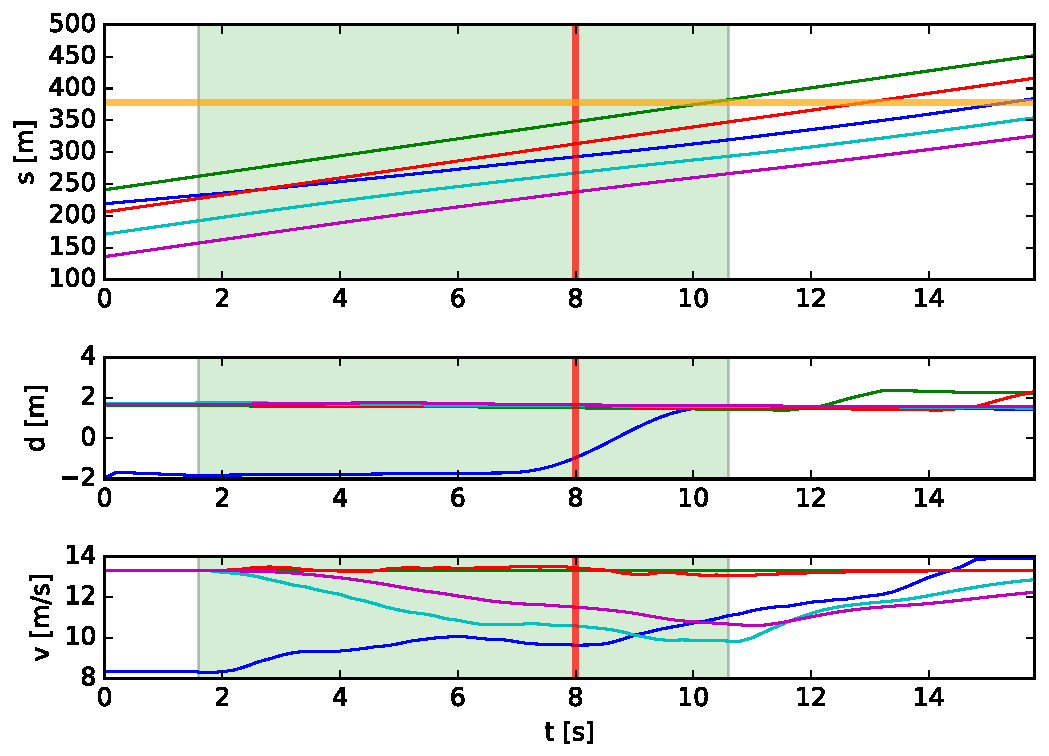
\includegraphics[width =  0.63 \textwidth]{30_kmh.pdf}
        \label{30kmh}
    }
    \subfigure[25 km/h]{
        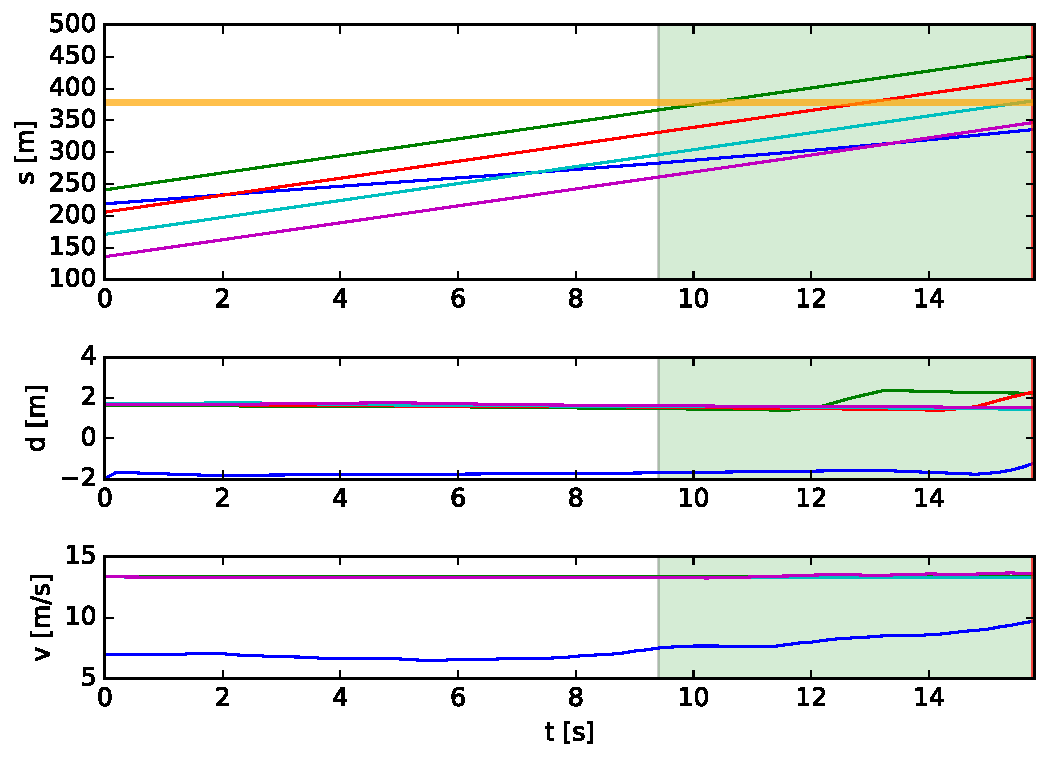
\includegraphics[width =  0.63 \textwidth]{25_kmh.pdf}
        \label{25kmh}
    }
    \caption[Verschiedene Anfangsgeschwindigkeiten]{Fahrstreifenwechsel bei verschiedenen Anfangsgeschwindigkeiten des Ego"=Fahrzeuges. F\"ur die Legende sei auf Abbildung~\ref{zweiFahrzeugeEgo} verwiesen.}
\end{figure}




\subsection{Fortlaufende Neuplanung}
\label{sec:AuswertungNauplanung}
In Kapitel~\ref{sec:einzelPlanungsschritt} konnte gezeigt werden, dass durch den vorgestellten Ansatz bei einem einzelnen Planungsschritt eine kooperative L\"osung gefunden werden kann.
Dabei wird ein kooperatives Verhalten der anderen Verkehrsteilnehmer angenommen.
Es soll nun \"uberpr\"uft werden, ob der Ansatz auch bei einer fortlaufenden Neuplanung zu einer sicheren, komfortablen und kooperativen Fahrstreifenwechseltrajektorie f\"uhrt.
Dazu wird zuerst von einem kooperativen Verhalten der anderen Verkehrsteilnehmer ausgegangen.
Anschlie{\ss}end wird \"uberpr\"uft zu welchem Ergebnis ein egoistisches Verhalten der anderen Verkehrsteilnehmer f\"uhrt.
Hierf\"ur wurde erneut ein Szenario mit zwei Fahrzeugen auf dem Zielfahrstreifen gew\"ahlt (siehe Abbildung~\ref{fig:two_veh_scene}).
Es wird angenommen, dass ein Planungsschritt in einer Zeit kleiner als \gls{symb:t_verarb} berechnet werden kann. 
Vom aktuellen Zeitpunkt  \gls{symb:t_jetzt} bis zum Zeitpunkt \gls{symb:t_jetzt} + \gls{symb:t_verarb} folgt Ego"=Fahzeug exakt der Trajektorie aus dem vorherigen Zeitschritt.
Anschlie{\ss}end steht eine neue Trajektorie zur Verf\"ugung.
Zu Beginn jedes Planungsschrittes ist die aktuelle Position aller Fahrzeuge bekannt.
Die Planung wird nicht mehr ver\"andert, nachdem dieser eingeleitet wurde.

\minisec{Neuplanung bei kooperativem Verhalten}
Es wird zuerst davon ausgegangen, dass die Fahrzeuge auf dem Zielfahrstreifen ein kooperatives Verhalten zeigen.
Dazu wird das Ergebnis aus dem ersten Planungsschritt als Verhalten der Fahrzeuge auf dem Zielfahrstreifen angenommen.


Das Ergebnis der Simulation ist in Abbildung~\ref{Replan} dargestellt.
Es ist ein \"ahnliches Trajektorienset wie bei einem einzelnen Planungsschritt zu erkennen.
Das Ego"=Fahrzeug sch\"atzt das kooperative Verhalten der Fahrzeuge auf dem Zielfahrstreifen richtig ein und f\"ahrt in die L\"ucke zwischen den Fahrzeugen auf dem Zielfahrstreifen ein.
Da die L\"osung des Multi-Agenten-Optimierungsproblems durch den randomisierten L\"osungsansatz nur angen\"ahert wird entspricht das Verhalten der Fahrzeuge, au{\ss}er im ersten Planungsschritt, nie exakt der Bewegungspr\"adiktion des Ego"=Fahrzeuges.
Trotz dieser Abweichung wird von dem vorgestellten Ansatz eine Trajektorie generiert, bei der auf das kooperative Verhalten der anderen Verkehrsteilnehmer reagiert wird und diese Verhalten f\"ur eine Fahrstreifenwechsel genutzt wird.
Dies zeigt, dass der Ansatz zu einem kooperativen Ergebnis f\"uhrt, solange sich die anderen Fahrzeuge \"ahnlich zur Bewegungspr\"adiktion verhalten.
Eine Bildabfolge des kooeprativen Fahrstreifenwechsels bei fortraufender Neuplanung ist im Anhang im Abbildung~\ref{fig:abfolgecoop} zu sehen.


\minisec{Neuplanung bei egoistischem Verhalten}
Es soll abschlie{\ss}end \"uberpr\"uft werden, wie das Ego"=Fahrzeug bei einer fortlaufenden Neuplanung auf ein egoistisches Verhalten der anderen Verkehrsteilnehmer reagiert.
Daf\"ur wird angenommen, dass die Fahrzeuge auf dem Zielfahrstreifen mit einer konstanten Geschwindigkeit fahren.

Die Ergebnisse sind in Abbildung~\ref{Replan_ego} dargestellt.
Die entsprechende Bildabfolge ist im Anhang in Abbildung~\ref{fig:abfolgeego} zu sehen.
Es ist zu sehen, dass der Ansatz bei einem egoistischen Verhalten der Fahrzeuge auf dem Zielfahrstreifen zu einem unerw\"unschten Fahrverhalten des Ego"=Fahrzeuges f\"uhrt.
Das Ego"=Fahrzeug geht davon aus, dass die Fahrzeuge auf dem Zielfahrstreifen sich kooperativ verhalten und die L\"ucke zwischen ihnen vergr\"o{\ss}ern.
Es erkennt das egoistische Fahrverhalten nicht und reagiert somit nicht darauf.
Dadurch kommt es beim Auffahren auf den Zielfahrstreifen zur deutlichen Unterschreitung von Sicherheitsabst\"anden.
Jeder Planungsschritt f\"uhrt zu dem Ergebnis, dass ein kooperatives Verhalten der Fahrzeuge auf dem Zielfahrstreifen zu geringen Gesamtkosten f\"uhrt.
Dadurch geht das Ego"=Fahrzeug bis zum Schluss davon aus, dass die Fahrzeuge auf dem Zielfahrstreifen die L\"ucke vergr\"o{\ss}ern werden um ihm das Auffahren auf den Zielfahrstreifen zu erleichtern.
Es z\"ogert den Fahrstreifenwechsel solange heraus, bis es am Ende des aktuellen Fahrstreifens angekommen ist.
Ein Anhalten auf dem aktuellen Fahrstreifen w\"urde dann eine unrealistische Verz\"ogerung erfordern.
Die L\"osung des Optimierungsproblems ergibt deshalb, dass ein Fahrstreifenwechsel die geringsten Kosten verursacht, selbst wenn dabei die Sicherheitsabst\"ande deutlich unterschritten werden. 
Es zeigt sich, dass der kooperative Planungsansatz bei einem unerwarteten Verhalten der anderen Fahrzeuge an seine Grenzen kommt.
In Kapitel~\ref{sec:diskussion} wird darauf eingegangen, wie diesen Grenzen entgegengewirkt werden kann.

\begin{figure}[!htbp]
    \centering
    \subfigure[Fortlaufende Neuplanung bei kooperativem Verhalten der Fahrzeuge auf dem Zielfahrstreifen]{
        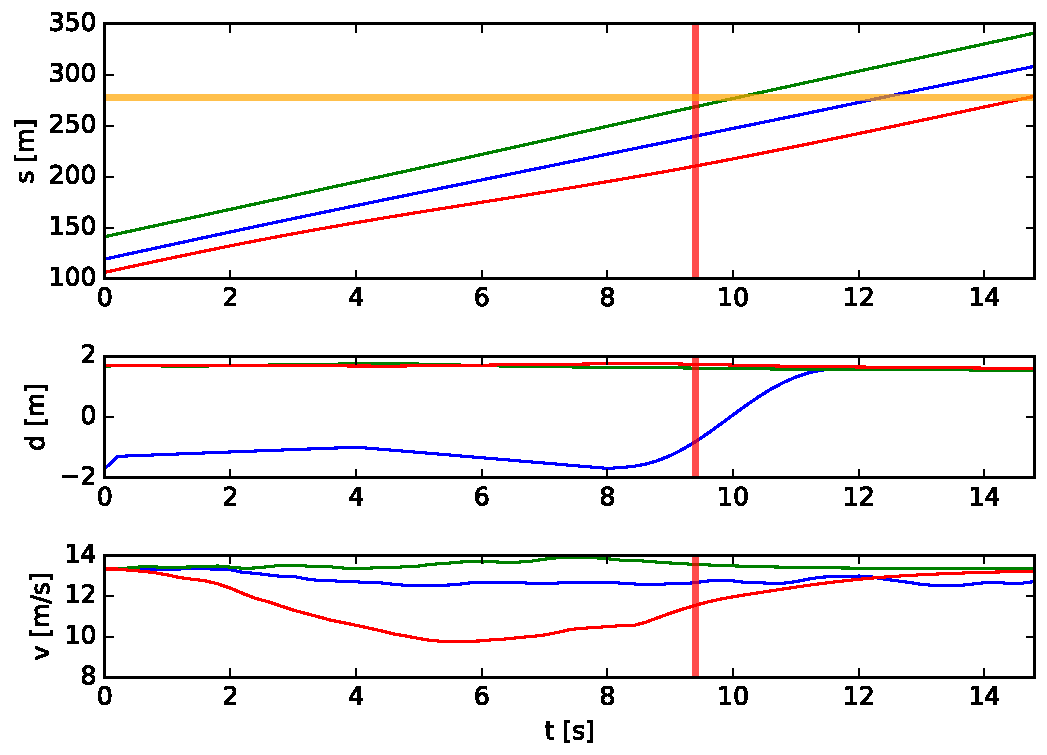
\includegraphics[width =  0.8 \textwidth]{Replan.pdf}
        \label{Replan}
    }
    \subfigure[Fortlaufende Neuplanung bei kooperativem Verhalten der Fahrzeuge auf dem Zielfahrstreifen]{
        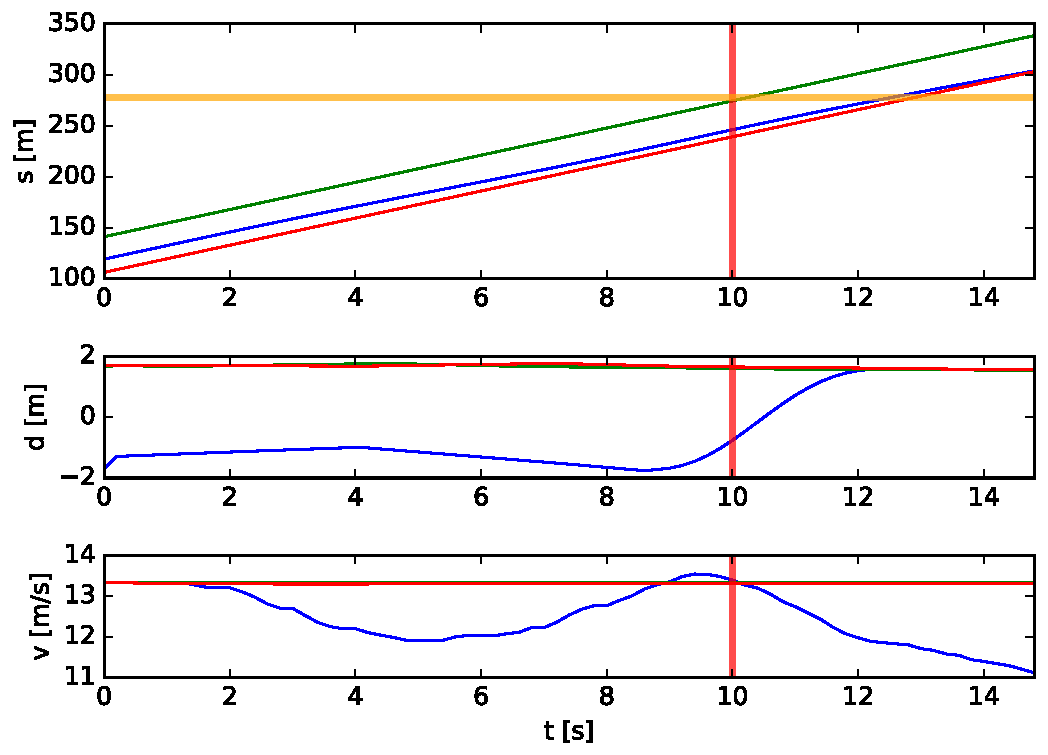
\includegraphics[width =  0.8 \textwidth]{Replan_ego.pdf}
        \label{Replan_ego}
    }
    \caption[Fortlaufende Neuplanung]{Fortlaufende Neuplanung. Die vertikale rote Line kennzeichnet den Zeitpunkt des Fahrstreifenwechsels \gls{symb:t_lc}.}
    \label{fig:Fort_Neuplanung}
\end{figure}




\section{Diskussion}
\label{sec:diskussion}
Es konnte gezeigt werden, dass der Ansatz zu einem Trajektorienset f\"uhrt, das einen kooperativen Fahrstreifenwechsel abbildet.
Es konnte auch gezeigt werden, dass der Ansatz zu einer sicheren und komfortablen Spruwechseltrajektorie f\"uhrt, solange sich die Fahrzeuge auf dem Zielfahrstreifen \"ahnlich zur Bewegungspr\"adiktion verhalten.
Das Verhalten des Ego"=Fahrzeuges und das erwartete Verhalten der anderen Verkehrsteilnehmer kann sich je nach Wahl der Parameter der Kostenfunktionale stark von einander unterscheiden.
Ob der Ansatz sich auch im realen Verkehr bew\"ahren kann h\"angt damit stark von den gew\"ahlten Parametern ab.

Das Kostenfunktional der anderen Fahrzeuge muss so bestimmt werden, dass es m\"oglichst gut ihr Verhalten widerspiegelt.
Da sich das Verhalten jedoch von Fahrer zu Fahrer unterscheidet, m\"usste auch das Kostenfunktional angepasst werden.
H\"aufig bleibt dem automatisierten Fahrsystem jedoch nur ein sehr kurze Zeitspanne um das Verhalten der Verkehrsteilnehmer zu beobachten.
Es ist nicht davon auszugehen, dass diese Zeit ausreicht um das Verhalten anderer Fahrzeuge zu analysieren und darauf beruhend ein angepasstes Kostenfunktional zu erstellen.

Eine M\"oglichkeit auf diesen Aspekt einzugehen ist, dass von einem allgemeinen Kostenfunktional ausgegangen wird.
Diese Kostenfunktional wird auf alle Fahrzeuge angewandt.
Es sollte deshalb m\"oglichst gut das allgemeine Fahrverhalten von nicht automatisierten Fahrzeugen repr\"asentieren.
Untersuchungen zur Generierung eines solchen Kostenfunktionals wurden von Tr\"unkle \cite{Trunkel} gemacht.
Da verschiedene Fahrsituationen ein unterschiedliches Verhalten fordern muss das Kostenfunktional noch entsprechend der Verkehrsregeln und der Ausgangssituation angepasst werden.
Verhalten sich die interagierenden Fahrzeuge \"ahnlich zu dem Fahrverhalten das durch das allgemeine Kostenfunktional ausgedr\"uckt wird, f\"uhrt der vorgestellte Planungsansatz zu einer kooperativen Fahrstreifenwechseltrajektorie.

In Kapitel~\ref{sec:AuswertungNauplanung} wurde jedoch auch gezeigt, dass der Ansatz an seine Grenzen ger\"at, sobald Fahrzeuge stark von dem angenommenen Verhalten abweichen.
Es wird deutlich, dass parallel zur kooperativen Planung weitere \"Uberpr\"ufungen stattfinden m\"ussen um auch bei unerwartetem Verhalten anderer Fahrzeuge ein sicheres Fahrverhalten zu garantieren.
In Naumann et al. \cite{Naumann2018} wird vorgeschlagen parallel zur kooperativen Planung eine \"Ubereinstimmungs\"uberpr\"ufung und eine Sicherheits\"uberpr\"ufung durchzuf\"uhren.
Bei der \"Ubereinstimmungs\"uberpr\"ufung wird abgesch\"atzt wie wahrscheinlich es ist, dass die anderen Fahrzeuge sich entsprechend der Bewegungspr\"adiktion verhalten.
Ergibt die \"Ubereinstimmungs\"uberpr\"ufung, dass sich ein Fahrzeug wahrscheinlich nicht kooperativ verhalten wird, kommt ein konservativer Ersatzplan zum Einsatz.
Bei einem Fahrstreifenwechsel w\"are ein konservativer Ersatzplan, dass das Fahrzeug auf dem aktuellen Fahrstreifen bleibt und seine Geschwindigkeit verringert.

In der Sicherheits\"uberpr\"ufung wird gepr\"uft ob sich das Fahrzeug in einem sicheren Zustand befindet.
Ist dies nicht der Fall wird ein Notfallplan durchgef\"uhrt.
Bei einem Fahrstreifenwechsel w\"are zu pr\"ufen ob zum Zeitpunkt des Fahrstreifenwechsels der Abstand zu den Fahrzeugen auf dem Zielfahrstreifen bereits gro{\ss} genug ist um einen sicheren Fahrstreifenwechsel zu garantieren.
Desweiteren sollte gepr\"uft werden bis zu welchem Zeitpunkt es noch m\"oglich ist mit einem sicheren Bremsman\"over bis zum Ende dem aktuellen Fahrstreifen zum Stehen zu kommen.
Ist zu diesem Zeitpunkt ein sicherer Fahrstreifenwechsel noch nicht garantiert sollte das entsprechende Bremsman\"over als Notfallplan ausgef\"uhrt werden.

In Kapitel~\ref{globaleLV} wurde darauf hingewiesen, dass ein randomisierter L\"osungsansatz der nach einer bestimmten Zeit oder Anzahl an Stichproben abgebrochen wird nicht zur exakten L\"osung f\"uhrt.
Damit wird nicht die optimale Trajektorie des Ego"=Fahrzeuges ermittelt, sondern in den meisten F\"allen eine Trajektorie die \"ahnlich zu der optimalen Trajektorie ist.
Da laut \cite{Naumann2018} auch menschliche Fahrer nicht strikte Optimalit\"at anstreben, sondern vielmehr eine Trajektorie die nahe am Optimum ist, kann durch den Ansatz auch bei leichten Abweichungen vom Optimum ein menschen\"ahnliches Fahrverhalten widergespiegelt werden.
Es ist auch darauf hinzuweisen, dass ein probabilistischer Ansatz bei zwei Planungsschritten gleicher Ausgangssituation zu stark unterschiedlichen L\"osungen f\"uhren kann wenn die beiden L\"osungen \"ahnliche Kosten verursachen.
In einem solchen Fall ist davon auszugehen, dass auch f\"ur menschliche Fahrer nicht eindeutig ist welche Strategie zu bevorzugen ist und gegebenenfalls eine L\"osung gew\"ahlt wird die nicht dem globalen Optimum entspricht.
Der Ansatz spiegelt deshalb auch in solchen F\"allen ein menschliches Verhalten wider, selbst wenn die Trajektorie stark von der Optimaltrajektorie abweicht.
Eine solche uneindeutige Situation wird gel\"ost, indem die beteiligten Fahrzeuge zun\"achst die Strategie w\"ahlen die ihnen besser erscheint.
Dabei ist es nicht wichtig, dass die gew\"ahlte Strategie der optimalen Strategie entspricht, solange sie zu \"ahnlichen Kosten f\"uhrt.
Anschlie{\ss}end wird auf die sich neu ergebende Situation reagiert und die Planung wiederholt, bis die zu w\"ahlende Strategie eindeutig ist.
Bei automatisierten Fahrzeugen wird dieses Verhalten durch die fortlaufende Neuplanung erzeugt.


